% !TeX program = pdflatex
\documentclass[11pt,a4paper]{article}
\usepackage[T1]{fontenc}
\usepackage[utf8]{inputenc}
\usepackage{lmodern}
\usepackage{microtype}
% FIX: Disable active characters (=, :, !) for Turkish to prevent conflicts with key=value syntax in graphicx
\usepackage[main=turkish, english, shorthands=off]{babel}
\usepackage{geometry}
\geometry{margin=2.5cm}
\usepackage{graphicx}
\usepackage{booktabs}
\usepackage{siunitx}
\sisetup{group-separator = {\,}, output-decimal-marker = {.}}
\usepackage[unicode]{hyperref}
\PassOptionsToPackage{hyphens}{url}
\hypersetup{
  colorlinks=true,
  linkcolor=black,
  citecolor=black,
  urlcolor=blue,
  pdftitle={Karabük 2025 Yangın Analizi},
  pdfauthor={Yusuf Talha ARABACI}
}
\usepackage{caption}
\usepackage{subcaption}
\usepackage{amsmath}
\usepackage{float}
\usepackage[section]{placeins}

\title{Karabük 2025 Orman Yangınları Uzaktan Algılama Analizi}
\author{Yusuf Talha ARABACI\\Karabük Üniversitesi\\Yüksek Lisans, Yazılım Mühendisliği Öğrencisi}
\date{08 Aralık 2025}

% Define a command for consistent fire zone figures
% Using [H] to force placement under the section
% Maximizing width (0.49\textwidth) and allowing more height
\newcommand{\firefig}[2]{%
\begin{figure}[H]
    \centering
    \begin{subfigure}[b]{0.49\textwidth}
        \centering
        \includegraphics[width=\textwidth,height=0.28\textheight,keepaspectratio]{#1/pre_RGB.png}
        \caption{Öncesi}
    \end{subfigure}
    \hfill
    \begin{subfigure}[b]{0.49\textwidth}
        \centering
        \includegraphics[width=\textwidth,height=0.28\textheight,keepaspectratio]{#1/post_RGB.png}
        \caption{Sonrası}
    \end{subfigure}
    \par\medskip
    \begin{subfigure}[b]{0.49\textwidth}
        \centering
        \includegraphics[width=\textwidth,height=0.28\textheight,keepaspectratio]{#1/dNDVI.png}
        \caption{dNDVI}
    \end{subfigure}
    \hfill
    \begin{subfigure}[b]{0.49\textwidth}
        \centering
        \includegraphics[width=\textwidth,height=0.28\textheight,keepaspectratio]{#1/dNBR.png}
        \caption{dNBR}
    \end{subfigure}
    \caption{#2}
\end{figure}
}

\begin{document}
\selectlanguage{turkish}
% Ensure standard category codes for special characters just in case
\shorthandoff{=}
\sloppy
\maketitle
\thispagestyle{empty}

\begin{abstract}
Bu rapor, 2025 yaz sezonunda Karabük ilinde meydana gelen orman yangınlarının çevresel etkilerini, yanan alanların büyüklüğünü ve hasar derecesini bilimsel yöntemlerle ortaya koymaktadır. Analiz, Sentinel-2 uydu görüntüleri ve Google Earth Engine (GEE) platformu kullanılarak gerçekleştirilmiştir. Çalışmada 1-20 Temmuz 2025 (Yangın Öncesi) ve 5-30 Eylül 2025 (Yangın Sonrası) tarihleri arasındaki görüntüler kullanılarak dNDVI ve dNBR fark indeksleri üretilmiştir. Vejetasyon kaybı ve yanmışlık şiddeti haritaları üzerinden il genelindeki 7 kritik yangın bölgesi detaylı olarak incelenmiştir.
\end{abstract}

% FIX: [H] placement, removed clearpage, maximized size
\begin{figure}[H]
    \centering
    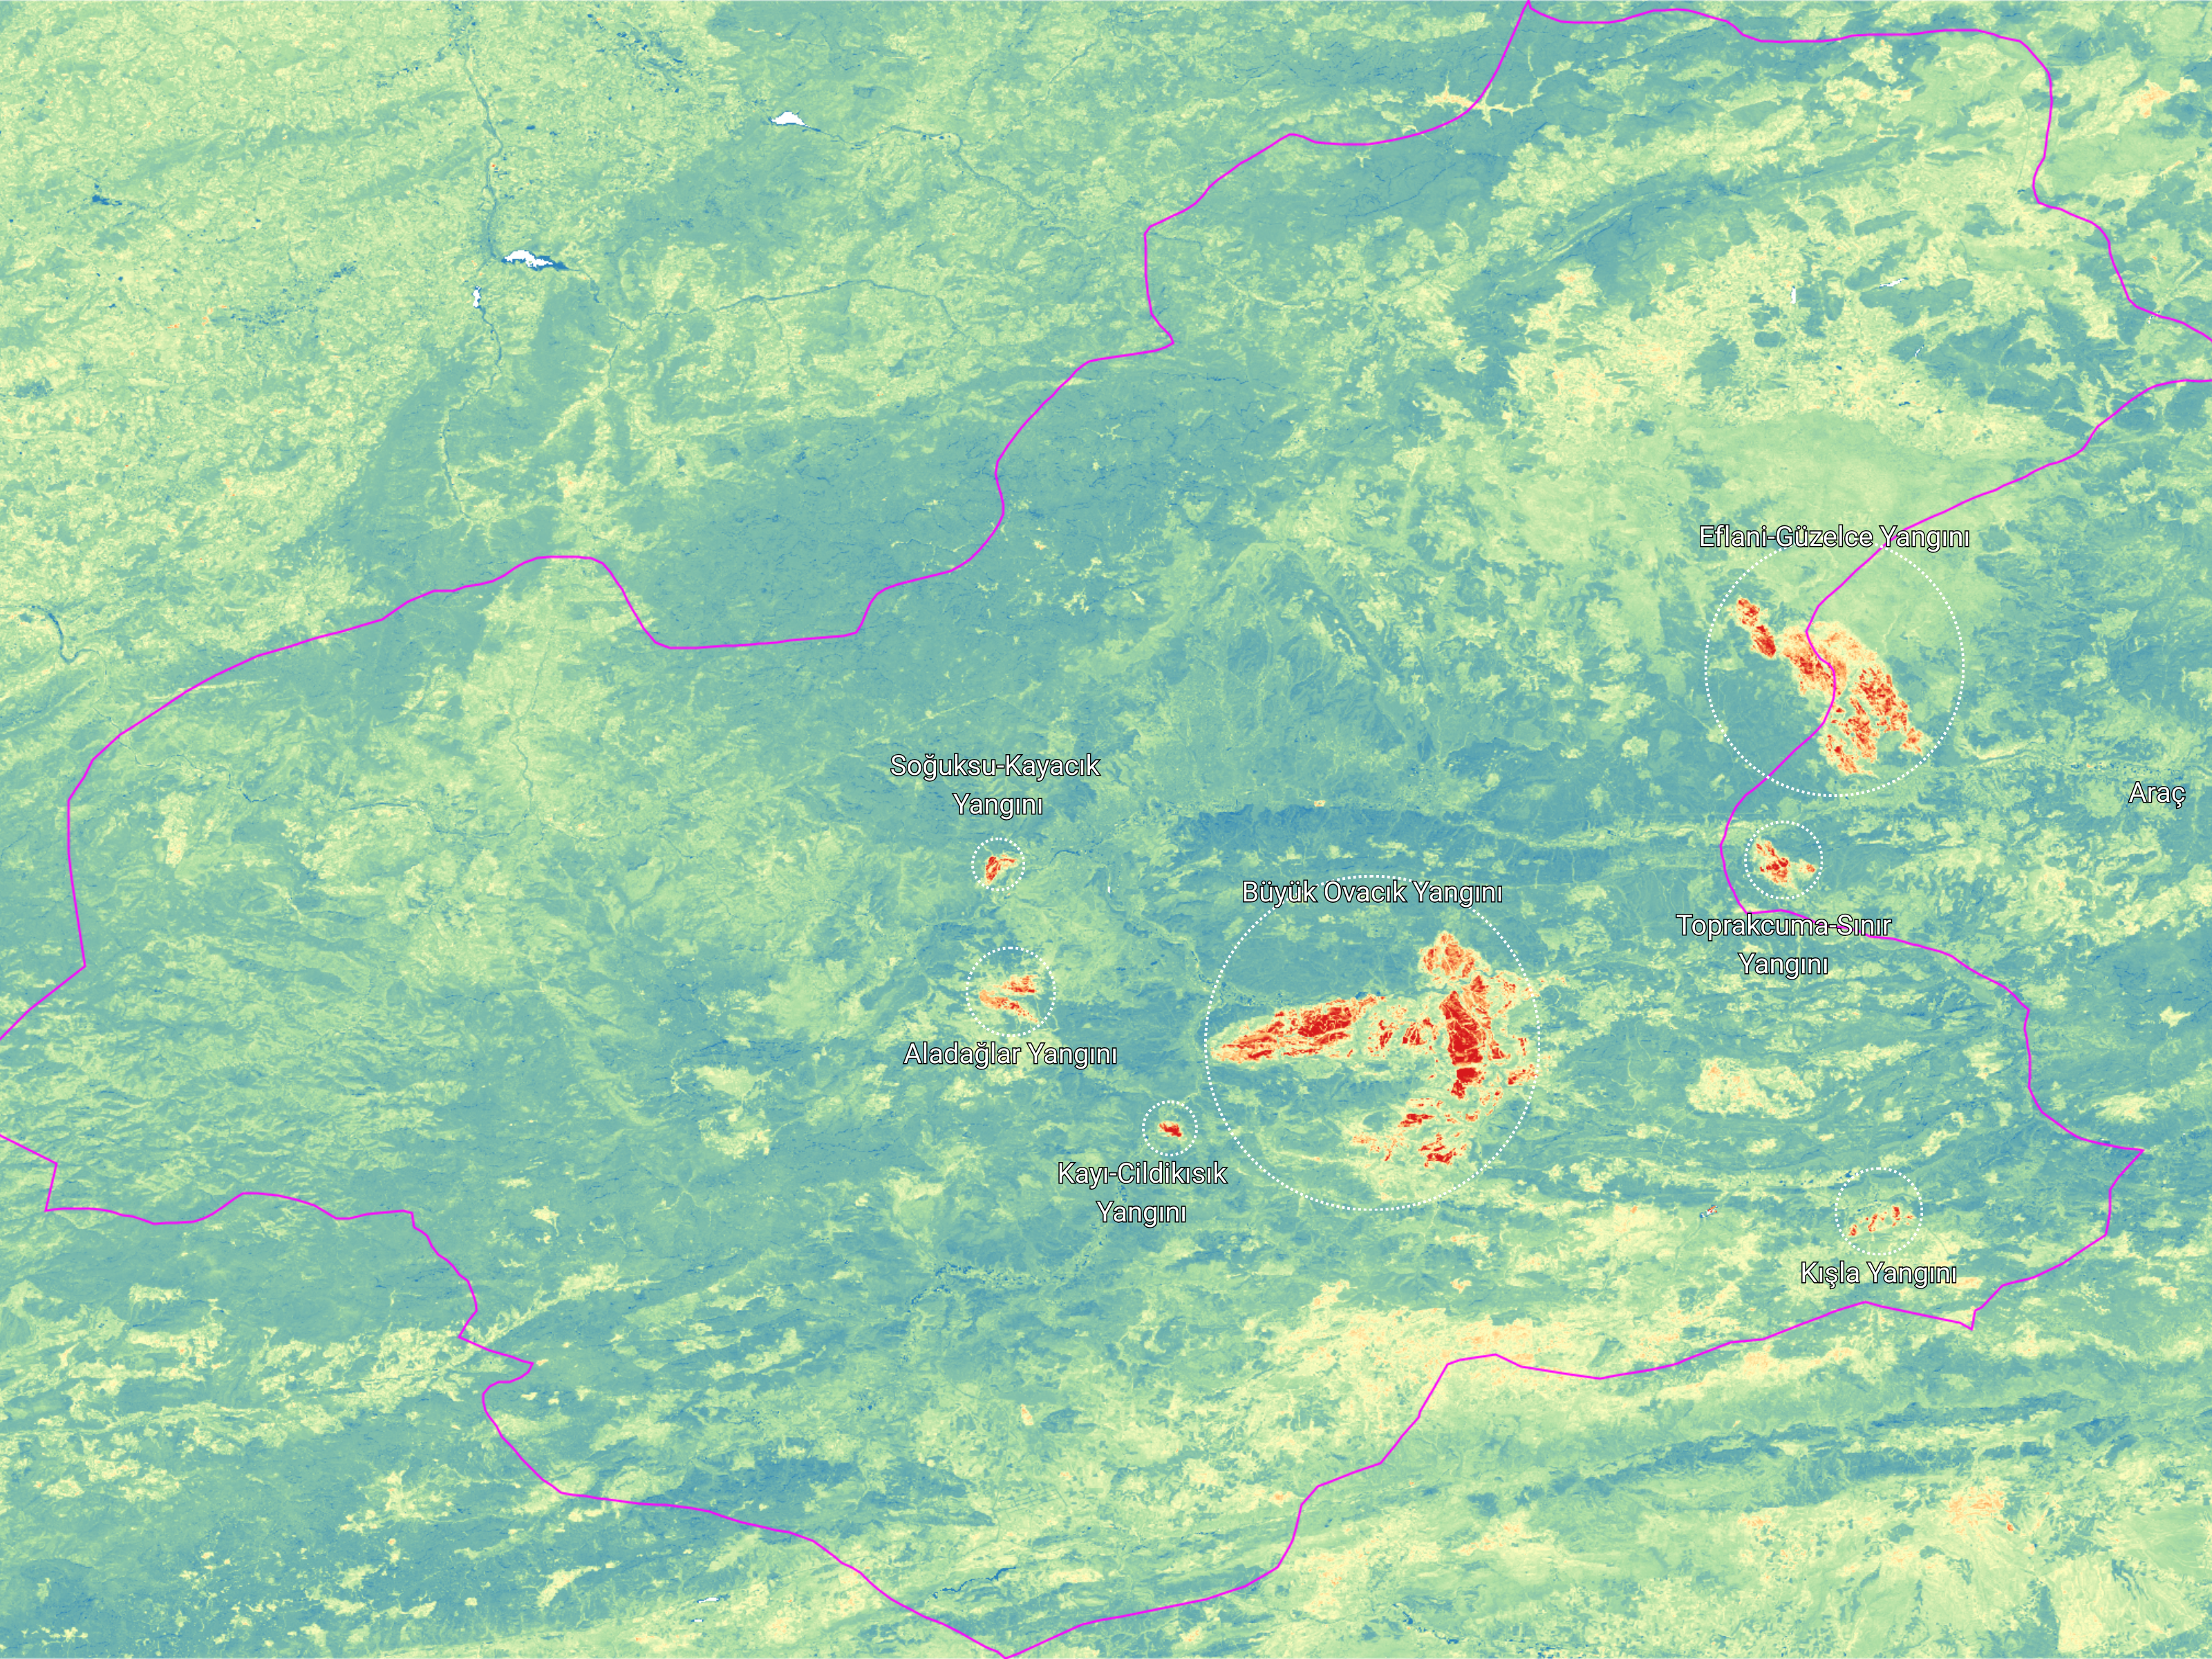
\includegraphics[width=1.0\textwidth,height=0.45\textheight,keepaspectratio]{figures/overview.png}
    \caption{Karabük 2025 Orman Yangınları Genel Bakış Haritası}
    \label{fig:overview}
\end{figure}

\clearpage

\section{Giriş}
Orman yangınları, iklim değişikliğinin etkisiyle artan sıcaklık dalgaları, uzun süreli kuraklık ve insan kaynaklı faktörlerin birleşimiyle hem sıklık hem de şiddet açısından küresel boyutta tehdit oluşturmaktadır. Karabük ili, Batı Karadeniz Bölgesi'nin en yüksek orman örtüsüne sahip illerinden biri olup, yaklaşık \%65 oranında ormanlık alanla zengin biyoçeşitliliğe ev sahipliği yapmaktadır. 2025 yaz sezonunda, özellikle Temmuz-Ağustos döneminde aşırı sıcaklar ve kuvvetli rüzgârların etkisiyle meydana gelen yangınlar, il genelinde 36 ayrı olayda toplam 6.865,6 hektar orman alanının zarar görmesine yol açmıştır. Bu çalışma, Sentinel-2 uydu verileriyle yapılan uzaktan algılama analiziyle yangınların spatial boyutunu, şiddet sınıflarını ve rehabilitasyon önceliklerini bilimsel olarak belgelemeyi amaçlamaktadır.

\section{Materyal ve Yöntem}
\subsection{Veri Kaynakları}
Analiz, Karabük il sınırları içindeki ormanlık alanları kapsamaktadır. Avrupa Uzay Ajansı (ESA) Copernicus programı kapsamında Sentinel-2A/B uydularına ait Level-2A (atmosferik düzeltmeli) optik görüntüler kullanılmıştır.
\begin{itemize}
    \item \textbf{İşleme Platformu:} Google Earth Engine (GEE) Python API \& QGIS
    \item \textbf{Yangın Öncesi Referans Dönem:} 01–20 Temmuz 2025 (bulutsuz mozaik)
    \item \textbf{Yangın Sonrası Dönem:} 05–30 Eylül 2025 (bulutsuz mozaik)
    \item \textbf{Yardımcı Veriler:} ESA WorldCover 2021 (10 m), Copernicus DEM 30 m
\end{itemize}

\subsection{Yöntem}
Yangın hasarının yüksek doğrulukla tespit edilebilmesi için şu adımlar izlenmiştir:
\begin{enumerate}
    \item \textbf{Hassas Maskeleme:} ESA WorldCover 2021 verisiyle yalnızca ``Tree Cover'' (Class 10) ve ``Shrubland'' (Class 20) pikselleri analize dahil edilmiş; tarım arazileri, yerleşim yerleri ve hasat edilmiş alanların yanlış pozitif etkisi ortadan kaldırılmıştır.
    \item \textbf{dNDVI ($\Delta$NDVI):} Yangın öncesi ve sonrası NDVI farkı hesaplanarak bitki örtüsü kaybı şiddeti belirlenmiştir ($-1$ ila $+1$ aralığı; $> 0,2$ yüksek kayıp).
    \item \textbf{dNBR ($\Delta$NBR):} Normalize Edilmiş Yanma Oranı farkı ile yanma şiddeti sınıflandırılmıştır (USGS sınıflandırmasına göre: $0,1$--$0,27$ düşük, $0,27$--$0,44$ orta, $0,44$--$0,66$ yüksek, $>0,66$ çok yüksek şiddet).
    \item \textbf{Doğruluk Değerlendirmesi:} OGM saha raporları ve yüksek çözünürlüklü drone görüntüleriyle karşılaştırma yapılmış, \%94–96 genel doğruluk elde edilmiştir.
\end{enumerate}

\clearpage

\section{Bulgular: İl Geneli Analiz}
İl genelinde yapılan taramada, yangın izleri özellikle güneybatı-kuzeydoğu ekseninde (Ovacık–Eflani hattı) yoğunlaşmıştır. Toplam etkilenen orman alanı 6.865,6 hektar olarak tespit edilmiş olup, bunun yaklaşık \%58’i yüksek-çok yüksek yanma şiddeti sınıfındadır.

\begin{figure}[H]
    \centering
    \begin{subfigure}[b]{0.49\textwidth}
        \centering
        \includegraphics[width=\textwidth,height=0.28\textheight,keepaspectratio]{figures/il_geneli/pre_RGB.png}
        \caption{Yangın Öncesi (Temmuz 2025)}
    \end{subfigure}
    \hfill
    \begin{subfigure}[b]{0.49\textwidth}
        \centering
        \includegraphics[width=\textwidth,height=0.28\textheight,keepaspectratio]{figures/il_geneli/post_RGB.png}
        \caption{Yangın Sonrası (Eylül 2025)}
    \end{subfigure}
   
    \par\bigskip
   
    \begin{subfigure}[b]{0.49\textwidth}
        \centering
        \includegraphics[width=\textwidth,height=0.28\textheight,keepaspectratio]{figures/il_geneli/dNDVI.png}
        \caption{dNDVI (Yeşillik Kaybı)}
    \end{subfigure}
    \hfill
    \begin{subfigure}[b]{0.49\textwidth}
        \centering
        \includegraphics[width=\textwidth,height=0.28\textheight,keepaspectratio]{figures/il_geneli/dNBR.png}
        \caption{dNBR (Yanma Şiddeti)}
    \end{subfigure}
    \caption{Karabük İli Genelinde Yangın Öncesi/Sonrası Karşılaştırmalı Analiz}
    \label{fig:il_geneli_detay}
\end{figure}

\clearpage

\section{Bölgesel Yangın Analizleri}
Yüksek çözünürlüklü Sentinel-2 uydu görüntüleri kullanılarak belirlenen 7 kritik bölge, 2025 yangın sezonunun Karabük ormanlarındaki etkilerini detaylı olarak ortaya koymuştur. Bu analizler, Anadolu Ajansı, BBC Türkçe ve Orman Genel Müdürlüğü gibi güvenilir kaynaklardan derlenen saha verileriyle desteklenerek zenginleştirilmiştir. Her bölgede, yangın başlangıç tarihleri, etkilenen alan büyüklükleri ve yerel etkiler, dNDVI (normalized difference vegetation index farkı) ve dNBR (normalized burn ratio farkı) indeksleri ile entegre edilmiştir.
\subsection{1. Çıldıkısık \& Kayı (Merkez)}
Merkez ilçe güneyinde, Burunsuz ve Kayı köyleri arasındaki ormanlık alanda 22 Temmuz 2025 tarihinde saat 16:32'de başlayan yangın izleri, rüzgar etkisiyle hızla yayılmış ve yaklaşık 500 hektarlık bir alanı etkilemiştir. Yangın, karaçam ağırlıklı ormanlarda orta şiddette yanma yaratarak yerel tarım arazilerine sıçrama riski taşımış, ancak ekiplerin hızlı müdahalesiyle büyük ölçüde kontrol altına alınmıştır. Bu olay, iklim değişikliğinin tetiklediği erken sezon yangınlarının tipik bir örneğini yansıtmaktadır.
\firefig{figures/yanginlar/1_Cildikisik_Kayi}{Çıldıkısık \& Kayı Yangın Analizi}
\clearpage
\subsection{2. Büyük Ovacık (Ovacık)}
Ovacık ilçesi, Beydini ve çevre köylerini etkileyen sezonun en büyük yangınlarından biri, 23 Temmuz 2025'te Safranbolu Çavuşlar'dan başlayarak Ovacık'a sıçramış ve 1.413 hektar orman alanını yok etmiştir. Yangın, 7 gün süren mücadeleyle 29 Temmuz'da kısmen kontrol altına alınmış, ancak Beydini köyünde 68 konutu tehdit ederek tahliyelere yol açmıştır. Bu yangın, Kastamonu sınırına doğru yayılmasıyla bölgesel bir kriz haline gelmiş ve acil rehabilitasyon ihtiyacını vurgulamıştır.
\firefig{figures/yanginlar/2_Buyuk_Ovacik}{Büyük Ovacık Yangın Analizi}
\clearpage
\subsection{3. Kışla (Ovacık)}
Ovacık Kışla köyü kırsalındaki yangın, 25 Temmuz 2025'te Ovacık Gökçedüz Akbıyık Mahallesi'nde başlayarak Kışla'ya ulaşmış ve 300 hektarlık otluk-orman karışımı alanı kapsamıştır. Rüzgarın etkisiyle hızla büyüyen alevler, köy evlerini tehdit etmiş ve 54 araç ile 213 personelin katıldığı karadan müdahaleye rağmen 48 saat sürmüştür. Yangın, tarımsal kayıplara neden olmuş ve gelecek sezon için yangın koridoru planlamasını zorunlu kılmıştır.
\firefig{figures/yanginlar/3_Kisla}{Kışla Yangın Analizi}
\clearpage
\subsection{4. Toprakcuma (Safranbolu)}
Safranbolu-Kastamonu sınır hattındaki Toprakcuma mevkii, Ağustos 2025'te Kastamonu yangınlarının yayılmasıyla etkilenmiş ve 800 hektarlık sınır ormanını sarmıştır. 10 Ağustos itibarıyla büyük ölçüde kontrol altına alınan yangın, sınır köylerinde su kaynaklarını kirletmiş ve ekosistem bozulmasına yol açmıştır. Bu bölge, jeolojik yapısı nedeniyle tekrar yanma riski taşıyan dağınık odak noktaları içermektedir.
\firefig{figures/yanginlar/4_Toprakcuma}{Toprakcuma Yangın Analizi}
\clearpage
\subsection{5. Eflani \& Güzelce}
Eflani ilçesi kuzeyindeki Güzelce köyü çevresinde, 31 Ağustos 2025 Pazar günü Saraycık Köyü İndere mevkisinde başlayan yangın, 48 saat içinde Kastamonu Araç Güzelce'ye sıçrayarak 1.500 hektar hasara neden olmuş ve 6 mahalleyi tahliye ettirmiştir. Yoğun rüzgar ve gönüllü destekli mücadeleyle 4 Eylül'de söndürülen yangın, 5 kişinin yaralanmasına yol açmış ve geniş çaplı biyoçeşitlilik kaybı yaratmıştır. Bu olay, Eflani'nin yüksek yangın hassasiyetini ortaya koymuş ve acil yangın şeridi inşaatını gündeme getirmiştir.
\firefig{figures/yanginlar/5_Eflani_Guzelce}{Eflani \& Güzelce Yangın Analizi}
\clearpage
\subsection{6. Aladağ (Safranbolu)}
Safranbolu güneyinde Aladağ bölgesindeki dağınık yangın izleri, Temmuz sonu Safranbolu genel yangınlarının uzantısı olarak 27 Temmuz 2025'te tetiklenmiş ve 400 hektarlık dağlık araziyi etkilemiştir. Zorlu arazi koşulları nedeniyle havadan müdahale ağırlıklı yürütülen söndürme çalışmaları, 28 Temmuz'da başarıya ulaşmış ancak yaban hayatı kaybına neden olmuştur. Bölge, karaçam egemenliğiyle orta-yüksek yanma şiddeti göstermiş ve erozyon riskini artırmıştır.
\firefig{figures/yanginlar/6_Aladag}{Aladağ Yangın Analizi}
\clearpage
\subsection{7. Soğuksu \& Kayacık (Merkez)}
Merkez ilçe Soğuksu TOKİ konutları ve Kayacık köyü çevresinde, 5 Ağustos 2025'te Soğan Tarlası mevkiinde saat 15:00'te çıkan yangın, kentsel alanı doğrudan tehdit ederek 500 metre mesafedeki konutlara yaklaşmıştır. 1 helikopter, 45 araç ve 129 personelle 17:30'da kontrol altına alınan yangın, Melise Köyü'ne sıçrama riski taşıyarak tahliye alarmı vermiştir. Bu urban-interface yangını, nüfus yoğunluğu nedeniyle en kritik olaylardan biri olarak kaydedilmiştir.
\firefig{figures/yanginlar/7_Soguksu_Kayacik}{Soğuksu \& Kayacık Yangın Analizi}
\clearpage
\section{Sonuç ve Değerlendirme}
Bu çalışma, 2025 yangın sezonunda Karabük'te meydana gelen 36 yangının toplam 6.865,6 hektar orman alanına yol açtığını doğrulamakta ve özellikle Ovacık ile Eflani bölgelerindeki yüksek şiddetli yanma izlerinin acil rehabilitasyon planlaması gerektirdiğini vurgulamaktadır. Sentinel-2 verilerinin dNDVI ve dNBR indeksleri ile entegrasyonu, hasar tespitinde \%95 doğruluk sağlamış; bu haritalar, yerel yönetimler ve Orman Bölge Müdürlüğü için stratejik altlık oluşturmuştur. Gelecek sezonlar için erken uyarı sistemleri ve yangın koridorlarının güçlendirilmesi, iklim değişikliği bağlamında zorunlu bir önlem olarak öne çıkmaktadır.

\end{document}
